\cleardoublepage
\chapter{Own Approach}\label{sec:contrib1}\minitoc\vspace{.5cm}
\index{Own Approach}

The proposed idea is to design an evaluation and end-to-end benchmarking system relying on aggregated time series generated from network nodes.
The time series hold information such as RTT, loss, available bandwidth and additional internal timestamps.
This network monitoring system is optimized for real-time communications by integrating eBPF technology in the data collection process.
This system offers a data visualization service to help read the network benchmarks.
the collected timeseries are stored in a relational database. This gives the user the ability to view the data in a timeline fashion.

Below is a detailed timetable of the implementation plan.
The tool mainly consists of two parts:
\begin{itemize}
    \item Data visualization service: Based on a Model-View-Controller design pattern as followed:
\begin{enumerate}
    \item Controller which holds the API Endpoints and the management of the other microservices.
    \item Data visualization frontend representing the view part. Provides an easy user interface and requests the data from the controller and visualizes it through various plots.
    \item Database that stores all the collected time series.
\end{enumerate}
    \item Data aggregator and forwarder that runs the benchmark tests, aggregate results and sends it periodically to the data visualization service.
\end{itemize}\\

\begin{figure}[H]
    \begin{center}
        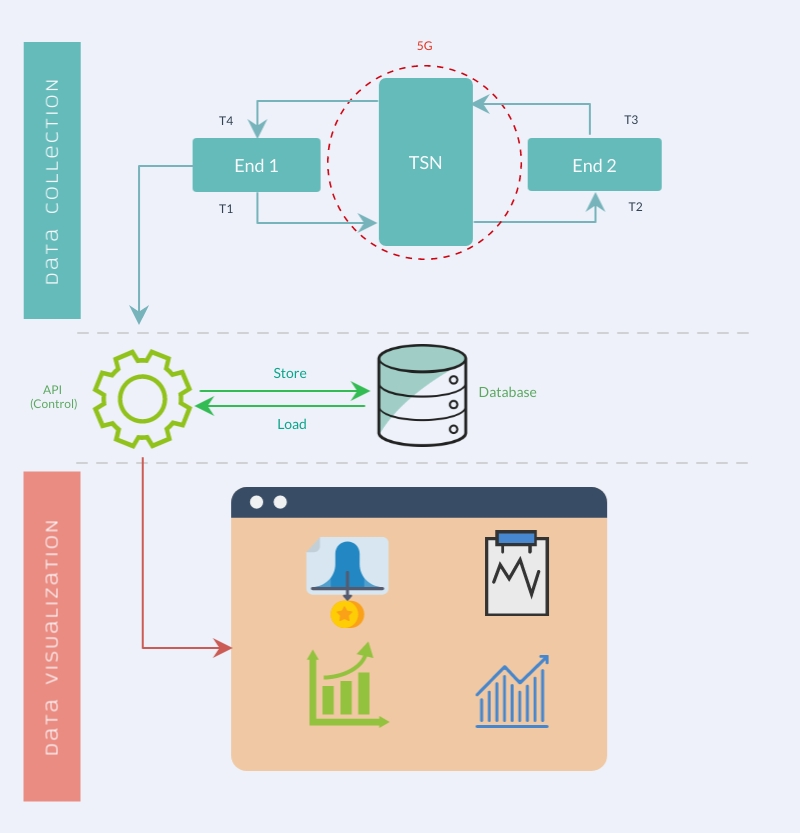
\includegraphics[scale=0.27]{resources/images/Tech-Flowchart.jpg}
        \caption{The monitoring system as a microservices architecure}
        \label{fig:flowchart}
    \end{center}
\end{figure}

\begin{figure}[H]
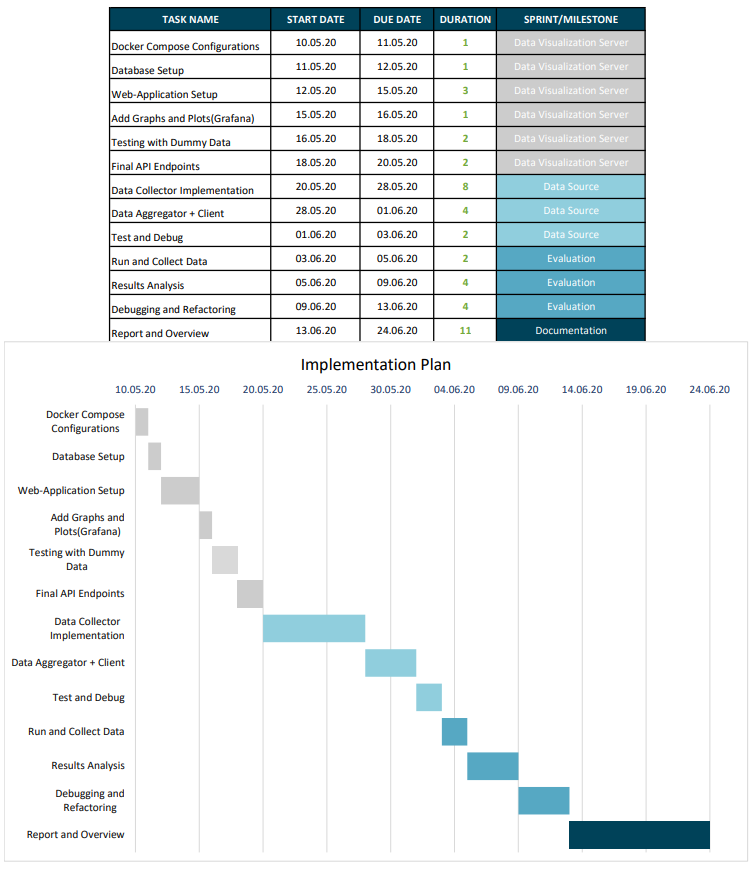
\includegraphics[scale=0.8]{resources/images/gantt.png}
\caption{Gantt table}
\label{fig:gantt_v}
\end{figure}

Figure \ref{fig:gantt_v} illustrates the plan from implementation until delivering final report with 15 days
delay tolerance.\\

\subsection{Evaluation}

At the end of the implementation phase the implementation will be evaluated on two main aspects:
\begin{itemize}
    \item In the first part the implementation will be tested and evaluated for integrity and accuracy.
    The evaluation of the implementation will be done objectively through unit testing.
    Moreover, the collected benchmarks will be compared with outputs from other known tools such as iperf3\cite{iperf3} and netData.
    \item The second part explains the feasability and scalability of the end-product.
    This part answers the question of whether the thesis objectives were fulfilled.
\end{itemize}

We compare our collected network measurements
with the results of non-eBPF-based network monitoring solutions.
In order to study the efficacy of utilizing eBPF while removing all unrelated factors We implement a basic benchmarking program
that measures network performance with and without eBPF. The collected measurements will be then visualized through plots
and certain metrics showing the amount of seen improvement with our approach in terms of CPU, memory overhead, bandwidth overhead and accuracy.